\chapter{Experiments} \label{chap:feasibility}

In this chapter two experiences in the field and the procedure followed in each case are reported. A feasibility study is introduced first in section \ref{sec:feasibility} and next, the real experiments for data acquisition are reported in section \ref{sec:experiment}.

\section{Feasibility study with children}\label{sec:feasibility}
It is imperative that a system which is ultimately to be used with children is tested in the hands
of children as soon as possible, to promote development of the design in the most appropriate
and necessary directions. To this end, a feasibility study was planned at a school on 30th of April
2015.

\subsection{Expected outcomes}

The desired outcome is the collection of all relevant information related with the robustness of the system and the experiment protocol, including

\begin{itemize}
\item the proper detection of the most relevant features captured to assess a measurement of the level of engagement and,
\item the implementation of an activity framework for easy addition of new activities.
\end{itemize}

This study should also allow the acquisition of a ground truth model of engagement using the manual assessment by two human observers during the interaction given an established criteria.

\subsection{Implementation of the activity framework}
The implementation has been split into two different ROS packages; the first one involves the management of activities. An activity can be writing (original CoWriter) or a simple story telling. And the second one, the adapting model behavior called \textit{emotionManager}. The execution of this second package is designed in such a way that becomes totally independent from the activities, and acts instead as a modifier inserting behaviors along the interaction. It is explained in detail in chapter \ref{chap:systemOverview}.

Following from previous tests conducted in the laboratory, a need for a higher level management of the interaction in the software was identified. Specifically, the need to control efficiently several activities and allowing it from external packages such as the emotion manager.

In order to reach this goal, the previous version of the state machine implemented to model the interaction \cite{hood2015children} was modified and extended to allow easy addition of activities as ROS nodes. This yields to include a high level controller for activity switching and pausing. For instance, it was a must to be able to switch from the original writing activity to a story telling since stopping the activities is not adequate. In the same way, it is also necessary to know which story has been told before.

Figure \ref{fig:stateMachine} shows an illustration of the state diagram of the interaction and management.

\begin{figure}[h!]
        \centering
        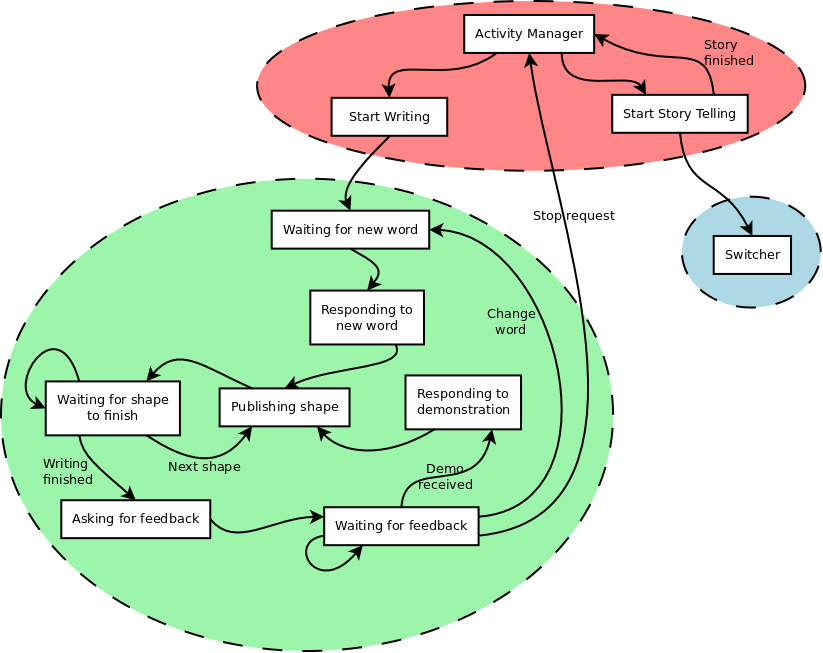
\includegraphics[width=0.75\textwidth]{figures/stateMachine.png}
        \caption{Framework implemented for in-situ studies}
        \label{fig:stateMachine}
\end{figure}

\subsection{Experimental design}

The experiment took place in Haut-Lac International School and 14 children in between 5 and 6 years took part of it. The children were organized in couples in order to find an emotional support with a known partner and allow a relaxed working environment.

\subsubsection{Scenario and procedure}
The experimental set-up (see figure \ref{fig:feasibility}) consists of the humanoid robot NAO, an external camera located between the feet of the robot and a tablet to interact with it. Additionally, during the experiment, two observers where located away from the interaction zone but having a face contact with the children interacting to assess engagement manually. Finally, the person guiding the activity or \textit{facilitator} was located at the left of the children. 

The two children in front of the robot interacting during 20 min each by turns. Each turn consisted on two activities; the original writing activity as an engaging one since intuitively is more interesting for children and a story telling as non-engaging, which was different for the two children. The main goal was to measure with the camera the features captured during both activities in order to find differences between them in terms of child attitude and behaviour.

\bigskip
\begin{figure}[h!]
        \centering
        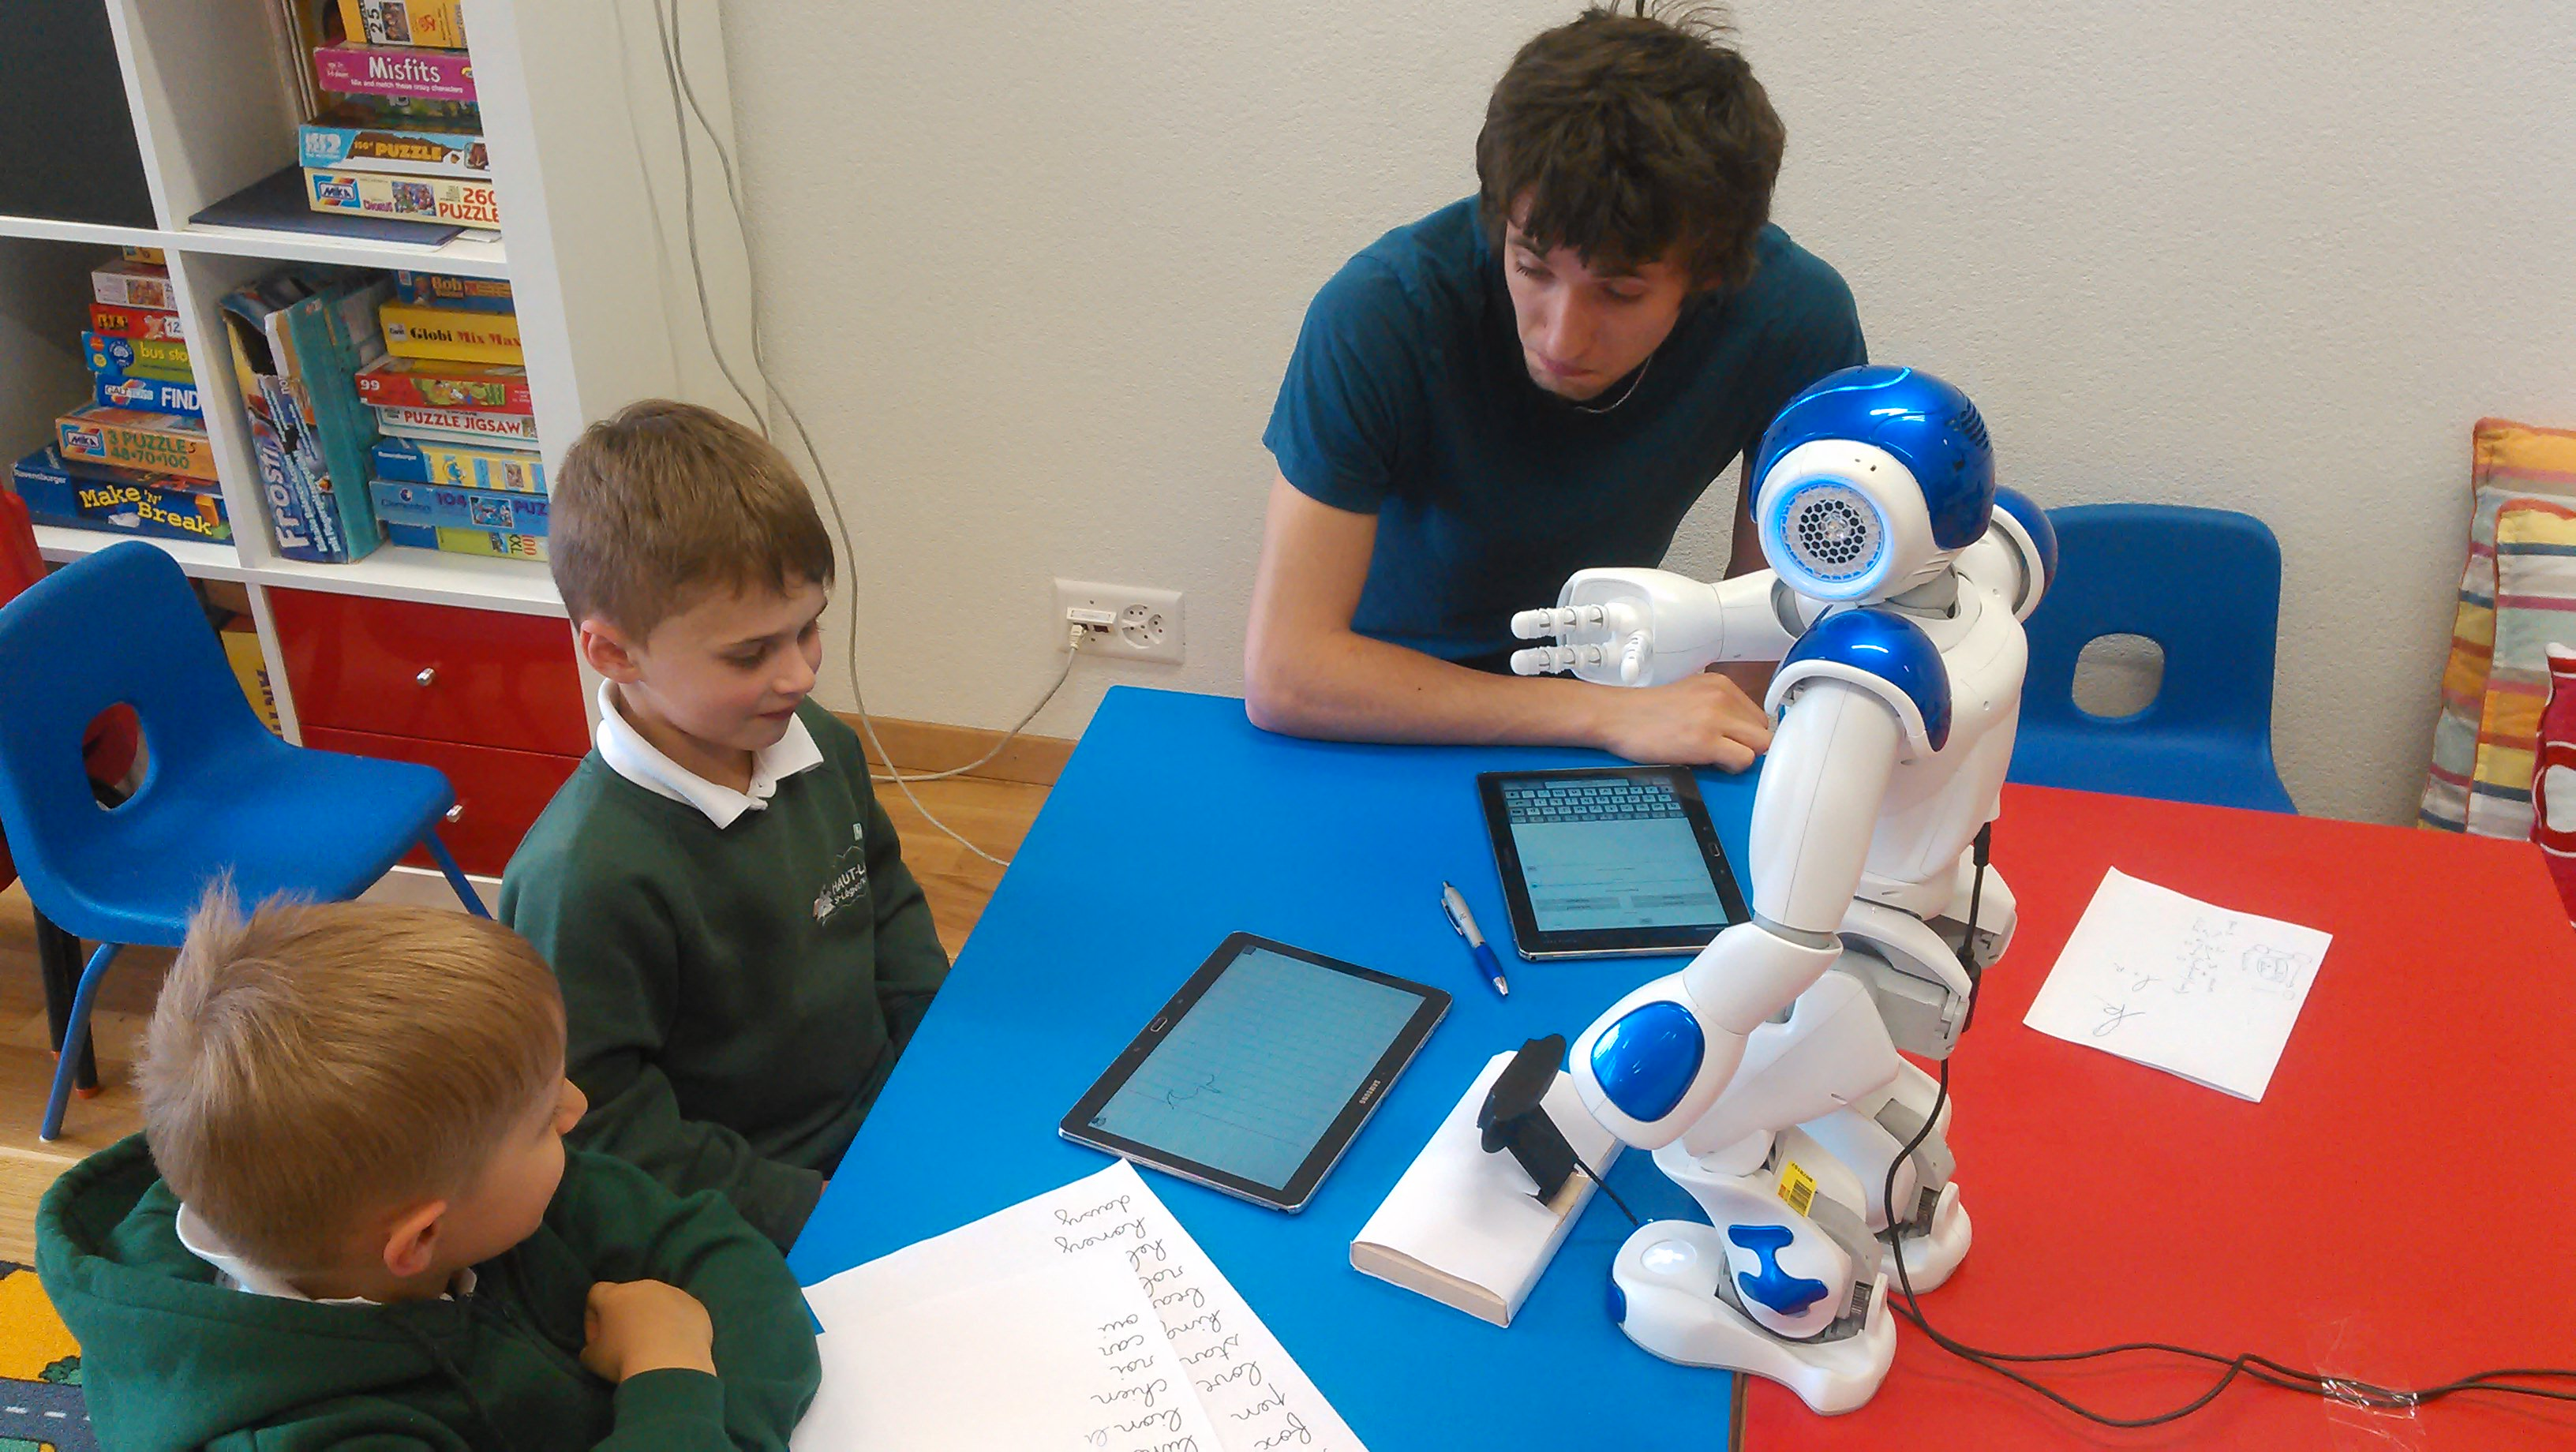
\includegraphics[width=0.7\textwidth]{figures/feasibility.jpg}
        \caption{Scenario during the feasibility test}
        \label{fig:feasibility}
\end{figure}

Therefore the goal was to obtain as much relevant data as possible in both, engaging and non engaging activities, to eventually be able to asses automatically when the child is one state or another.

\subsubsection{Measured variables} \label{measuredVariables}
During the activity the following variables were measured:

\begin{itemize}
\item Proximity to the region of interaction, robot and tablet.
\item Quantity of movement during both activities excluding the writing moments.
\item Gaze direction. Which side the child look to. 
\item Time response from the end of the robot demonstration till the stylus touch the tablet.
\item Time taken by the child to write the word.
\item Smile counter.

\end{itemize}
	

\subsubsection{Ground truth acquisition}
The ground truth is one of the most important parts of the data acquisition since it will be the reference point of the result analysis. As in many cases, it was necessary to acquire it during the experiment. In order to do that an Android ROS application (see figure \ref{fig:dataCollect}) was developed as a tool to help the assessment by the human observers.


\begin{figure}[h!]
        \centering
        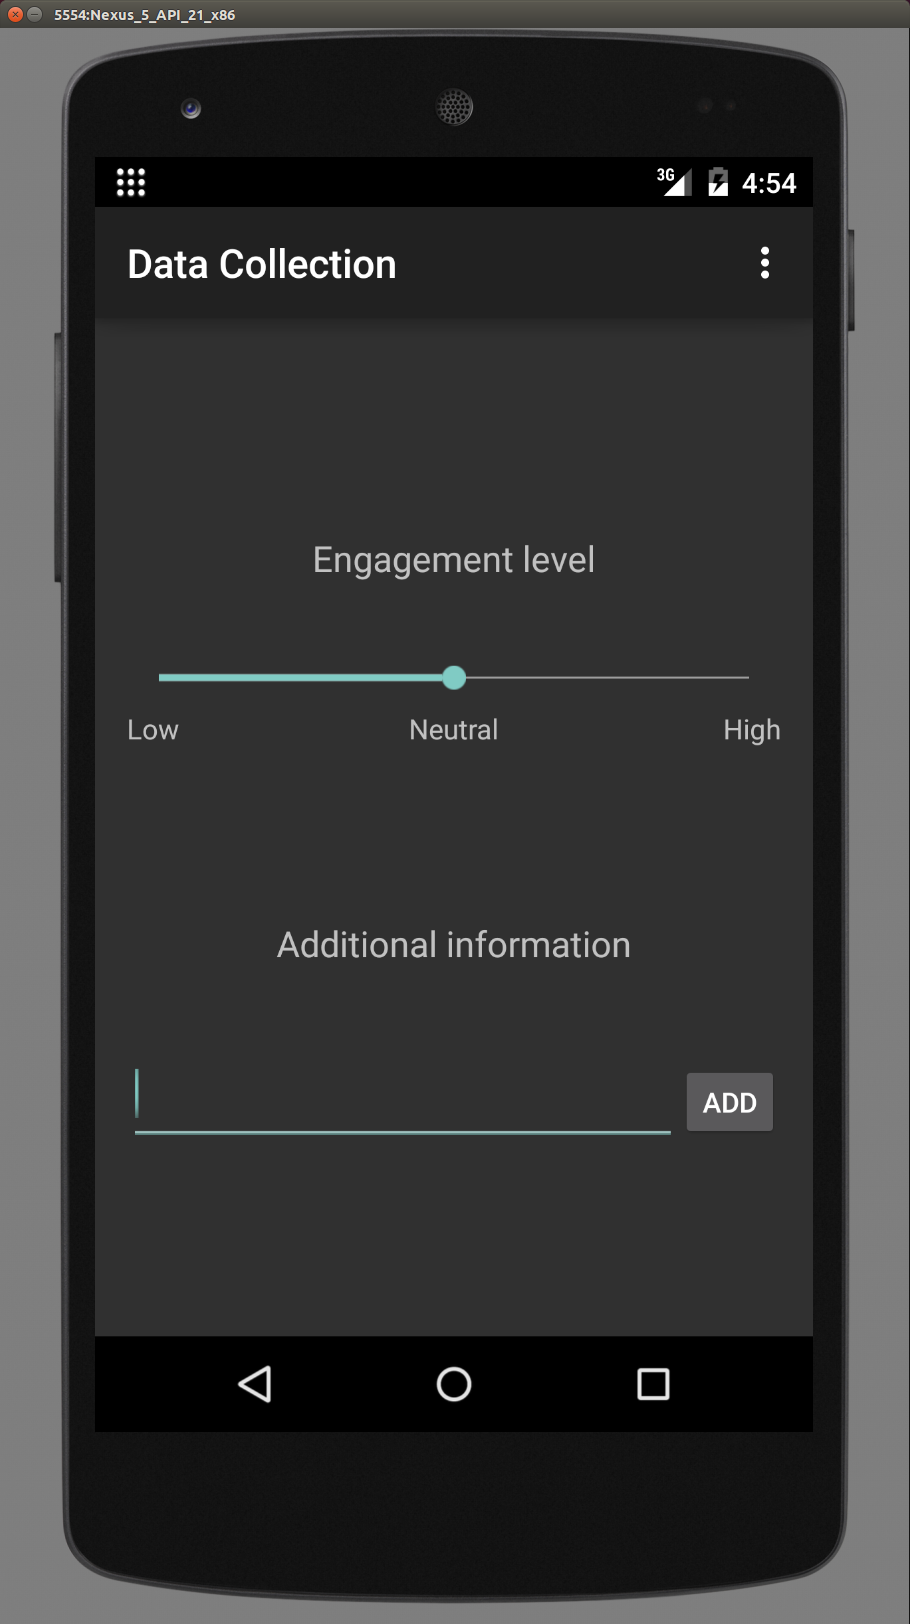
\includegraphics[width=0.3\textwidth]{figures/dataCollection.png}
        \caption{Engagement collection App for visual assessment}
        \label{fig:dataCollect}
\end{figure}


\subsection{Results}

We decided to provide a list of words to be chosen by the user in a sheet of paper. However, we quickly realized about the need of providing such words in a word selection application (see figure \ref{fig:wordSelector}) in order to smooth the interaction and the feeling of free choice. This simple Android ROS application publishes to the topic $ words\_to\_write $ when a button is pressed.

\begin{figure}[h!]
        \centering
        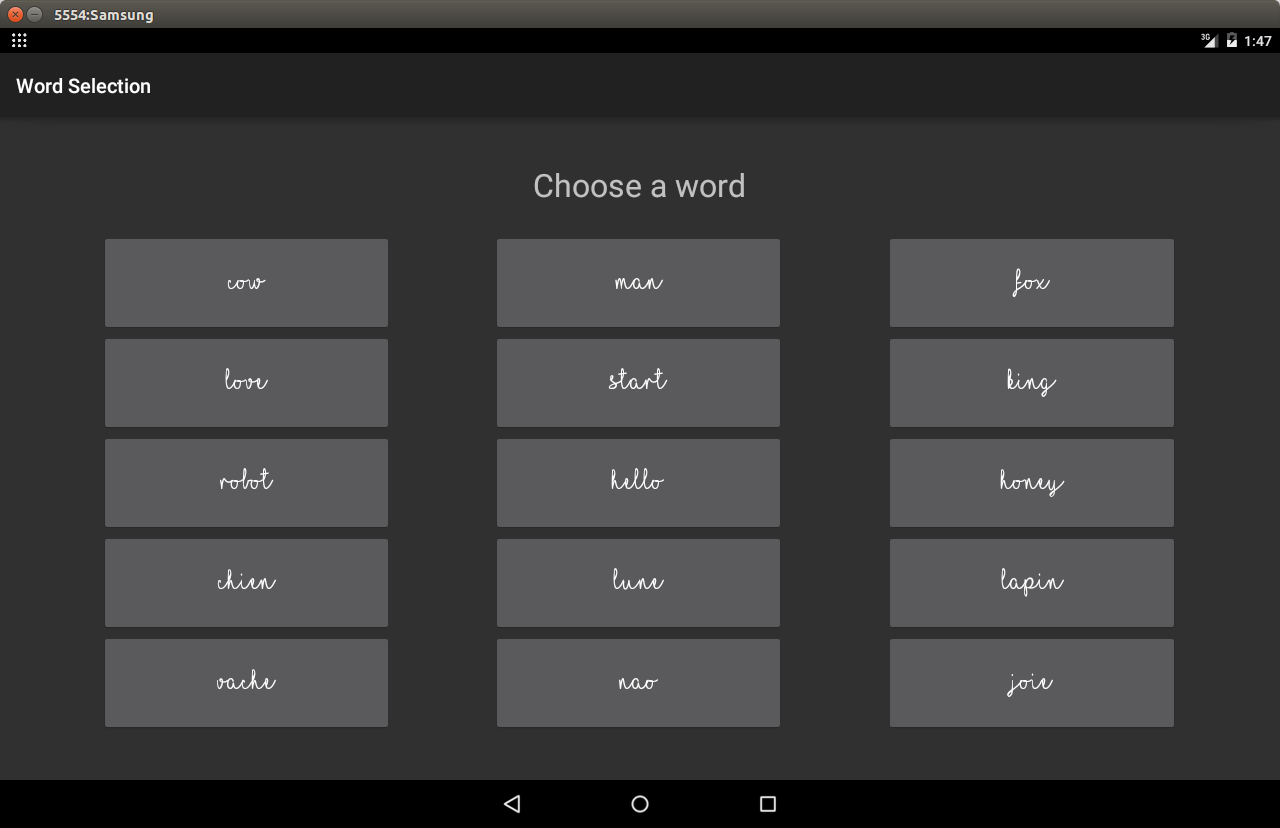
\includegraphics[width=0.7\textwidth]{figures/wordSelector.png}
        \caption{Word Selection App screenshot}
        \label{fig:wordSelector}
\end{figure}

Eventually, the data was acquired successfully and the application only crashed in two occasions during the 6 hours experiment. An experiment in a more controlled environment was scheduled and is presented in section \ref{sec:experiment}. However, several minor changes were reported and required to be fixed before that, such as:

\begin{itemize}
\item In order to correctly assess the level of engagement, it is necessary to minimize the human intervention. It turned to be a must that the experiment was for a single child. In addition, additional work was needed to better define the role of the facilitator and the human observers assessing the engagement.
\item The ground truth acquisition tool needed a simplification as well as a synchronization with the ROS master to be able to match the timestamps properly.
\item The age range was not the proper one in order to acquire writing samples and writing times to train the statistical engagement model proposed in Chapter \ref{chap:engagementModel}.
\item Several minor corrections related with the predefined speech of the robot and motion behaviour needed to be fixed.

\end{itemize}

\section{Data acquisition experiment} \label{sec:experiment} 
In this section the data acquisition through a formal experiment is explained in detail. However, the results extracted from this are discussed and analysed in detail in chapter \ref{chap:results}.
\subsection{Motivation}
After the feedback acquired in the first intervention through the feasibility study and the changes applied, it was necessary to go back to the field to collect data such as: shape letters, time and writing responses, gaze directions, quantity of movement and proximity distances, with a more stable system and improved protocol.


\subsection{Expected outcomes}

The desired outcome is the collection of all relevant information cited in section \ref{measuredVariables}, possibly related with the level of engagement, in order to tune the system to be able to give suggestions allowing long-term use with children. However, it also includes

\begin{itemize}
\item autonomous adaptive behaviours based on real-time information,
\item the data acquisition to detect correlations between the features tracked and the level of engagement and,
\item the acquisition of a ground truth model using the visual assessment of two observers during the interaction.

\end{itemize}

\subsection{Experimental design}
In this case, the experiments were scheduled in the International School of Geneva on June 5th, 2015 and 6 participants were involved.

\subsubsection{Scenario and procedure}
The experimental set-up (see figure \ref{fig:experiment}) consists of the humanoid robot NAO, an external camera located in the base of the robot and two tablets to interact with the robot: One where the CoWriter displays and collects the user demonstrations, and another one to select the word to write. In similar manner as in the feasibility study, the two observers where located away from the interaction zone but having a face contact with the children interacting. Finally, the person guiding the activity or \textit{facilitator} was located at the left of the children. 

\begin{figure}[h!]
        \centering
        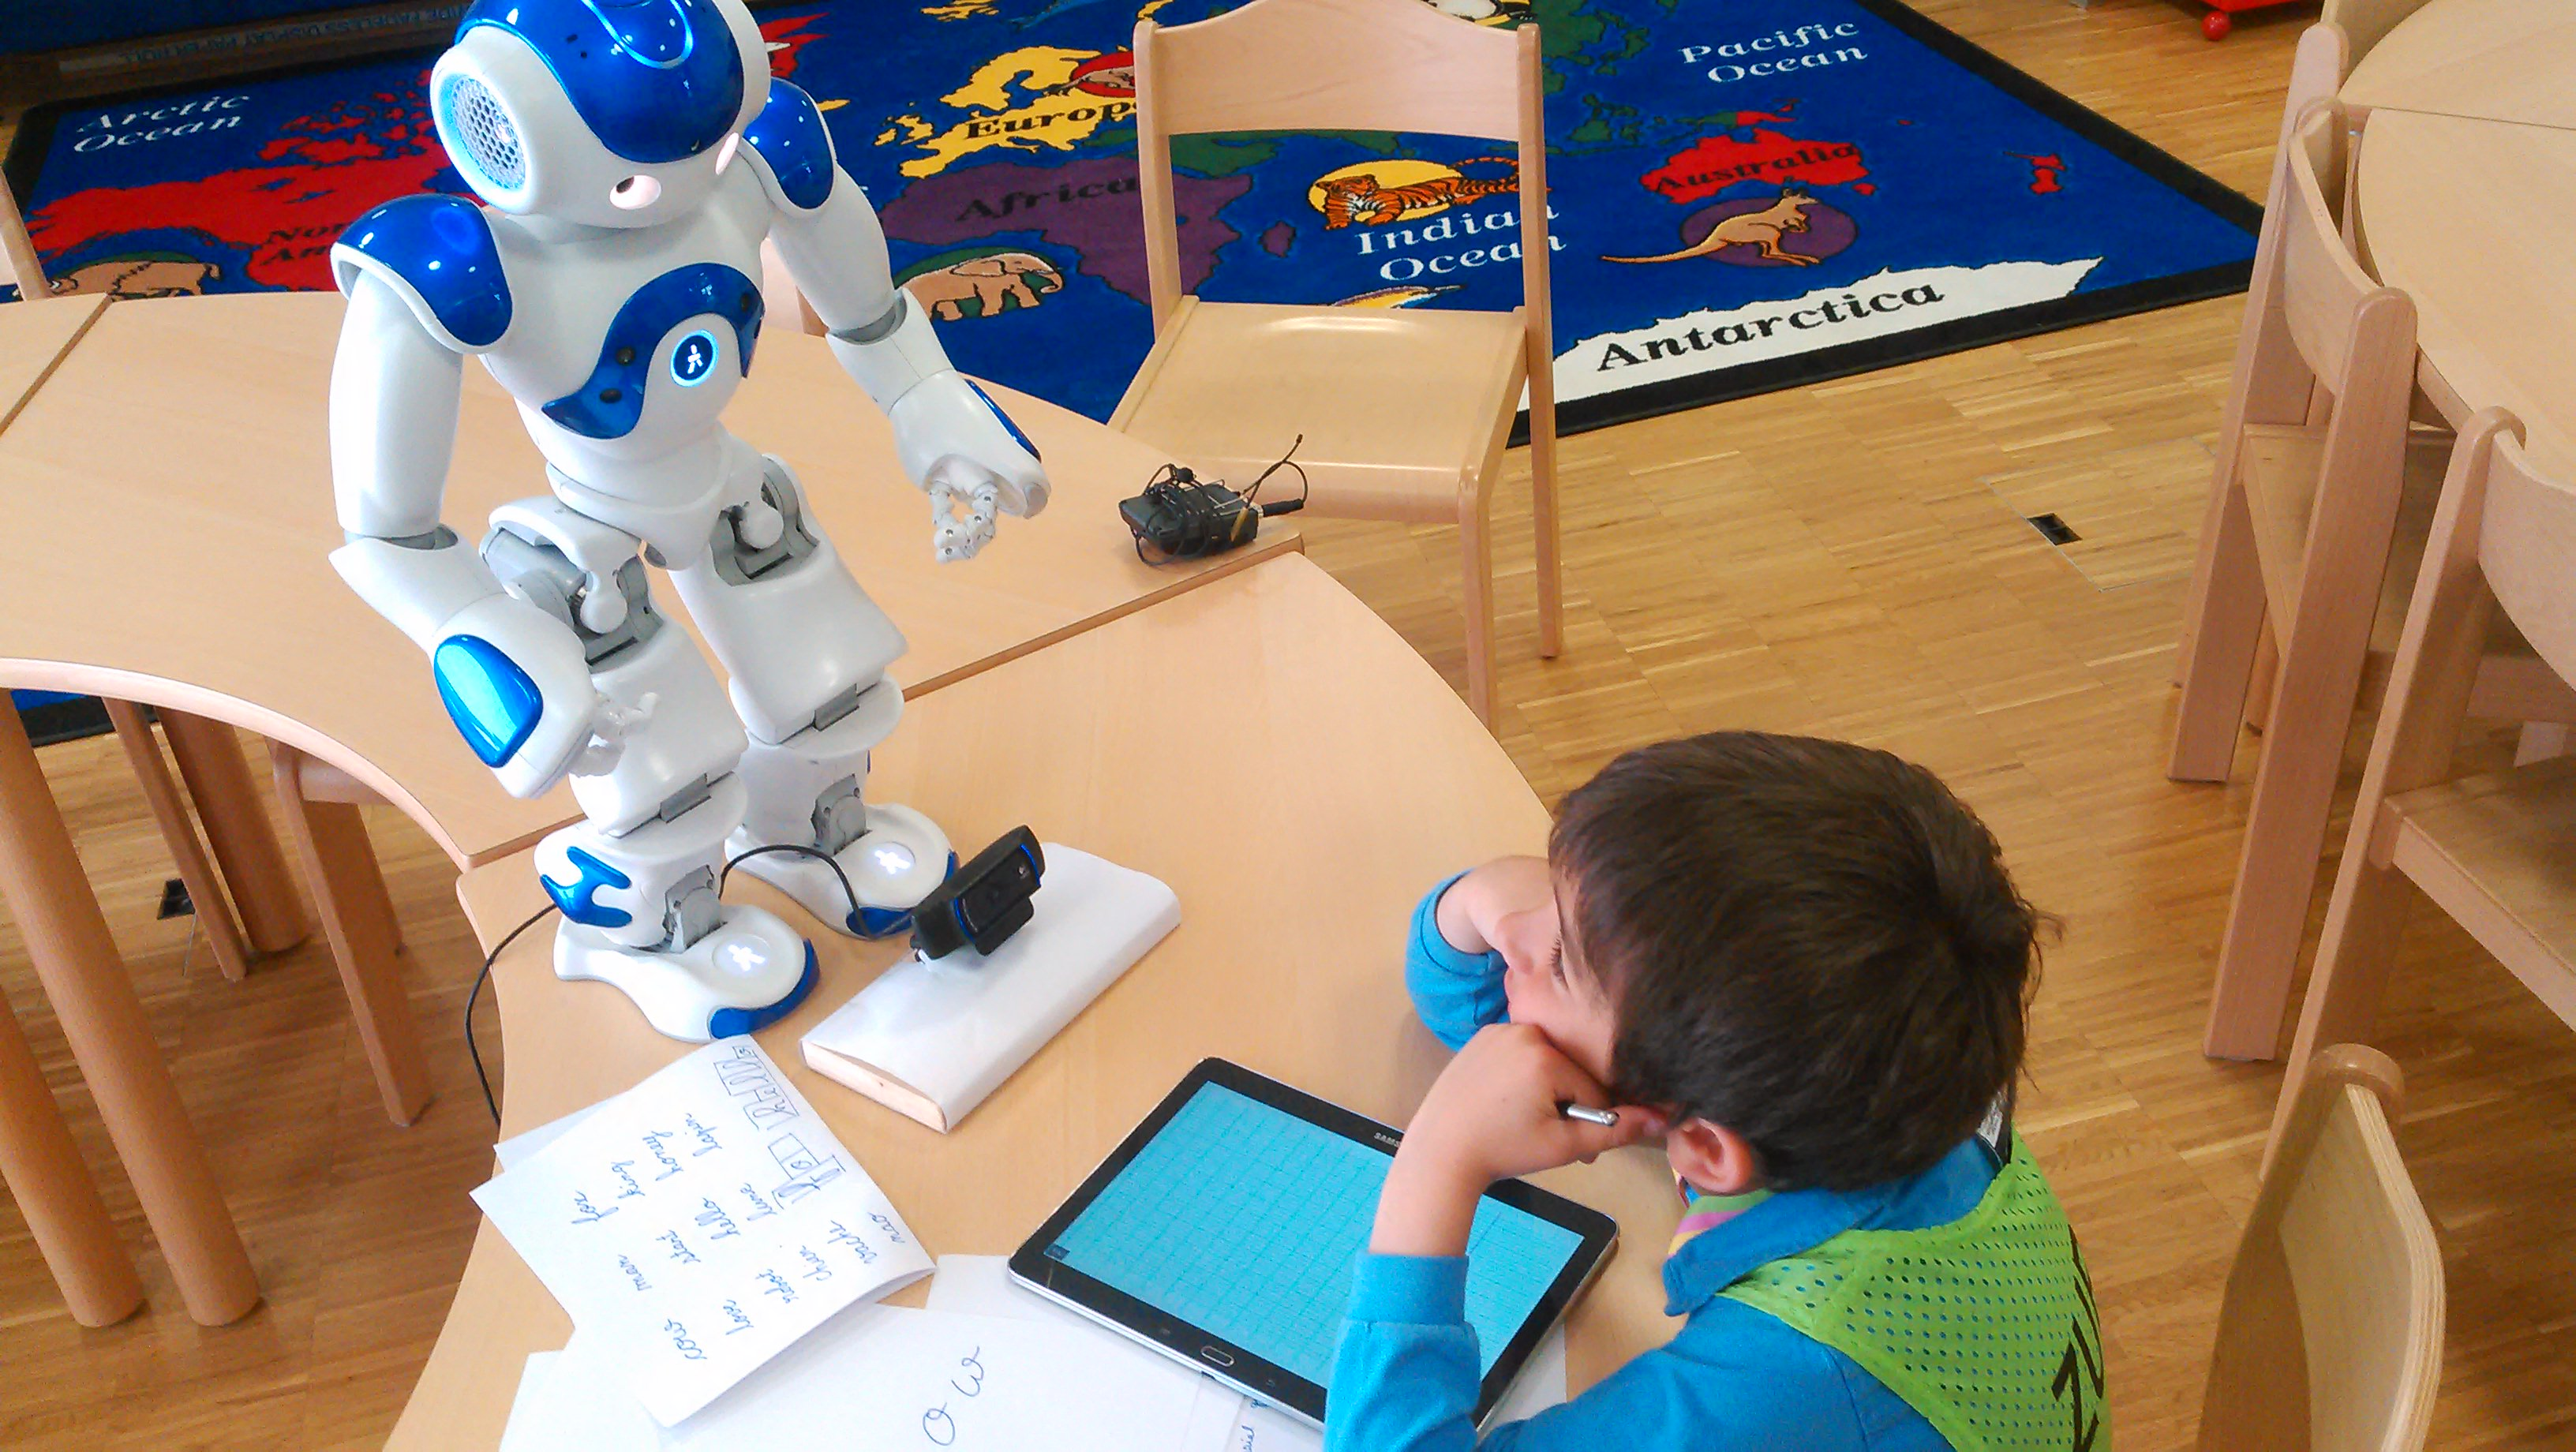
\includegraphics[width=0.7\textwidth]{figures/experiment.jpg}
        \caption{Redefined scenario during the experiments.}
        \label{fig:experiment}
\end{figure}

In this case, only one child interacted with the robot for 20 min. During this time, two activities were run; the original CoWriter (writing activity) as engaging task and the story telling as non-engaging. During this time the variables measured were the same as in section \ref{measuredVariables}.

